\documentclass[aspectratio=169]{beamer}
\usetheme{Madrid}

\title{Good Course Design and CS Materials}
\subtitle{}
\author{Kalpathi Subramanian$^1$, Erik Saule$^1$, Jamie Payton$^2$, and Matthew Mcquaigue$^1$ \\\texttt{krs@uncc.edu}, \texttt{esaule@uncc.edu}, \texttt{payton@temple.edu}, \texttt{mmcquaig@uncc.edu}}
\institute{$^1$The University of North Carolina at Charlotte\\$^2$Temple University}
\date{SIGCSE 2022}

\setbeamertemplate{footline}

\usepackage{hyperref,graphicx}
\usepackage{subfloat}

\beamertemplatenavigationsymbolsempty % remove navigation symbols
\begin{document}


\begin{frame}
\titlepage
\end{frame}


\AtBeginSection[]
{
    \begin{frame}
        \frametitle{Table of Contents}
        \tableofcontents[currentsection]
    \end{frame}
}

%
%
%
% CS Materials Piece
%
%
%


\section{Course design and alignment}

\subsection{Navigating Curriculum Guidelines}

\AtBeginSubsection[]
{
    \begin{frame}
        \frametitle{Table of Contents}
        \tableofcontents[currentsection,currentsubsection]
    \end{frame}
}


\begin{frame}
  \frametitle{Curriculum Guidelines}

  \begin{block}{What are they?}
    Usually they are recommendation of what should/could be taught across a program.

    Expressed in term of topics, learning outcome, and competencies. Not in term of courses.

    Usually make recommendation on how much one should learn in a
    particular topic, sometimes specified in number of hours.
  \end{block}


  \begin{block}{How can we use them?}
    Give us a reference of what we should/could be teaching.

    Am I covering all that? Should I? Why not?

    Give us a common language to communicate between instructors.
  \end{block}
\end{frame}

\begin{frame}
  \frametitle{General Guidelines: ACM/IEEE CS 2013}

  \begin{columns}
    
    \column{.45\linewidth}
    
  Structured in
  \begin{itemize}
  \item Knowledge Area
  \item Knowledge Unit
  \end{itemize}

  Topics and Learning Outcomes are classified as
  \begin{itemize}
  \item Tier-1
  \item Tier-2
  \item Elective
  \end{itemize}
  
  Other general guidelines:
  \begin{itemize}
  \item Data Science
  \item Computer Engineering
  \item Upcoming revised CS
  \end{itemize}
  
    \column{.53\linewidth}
    
  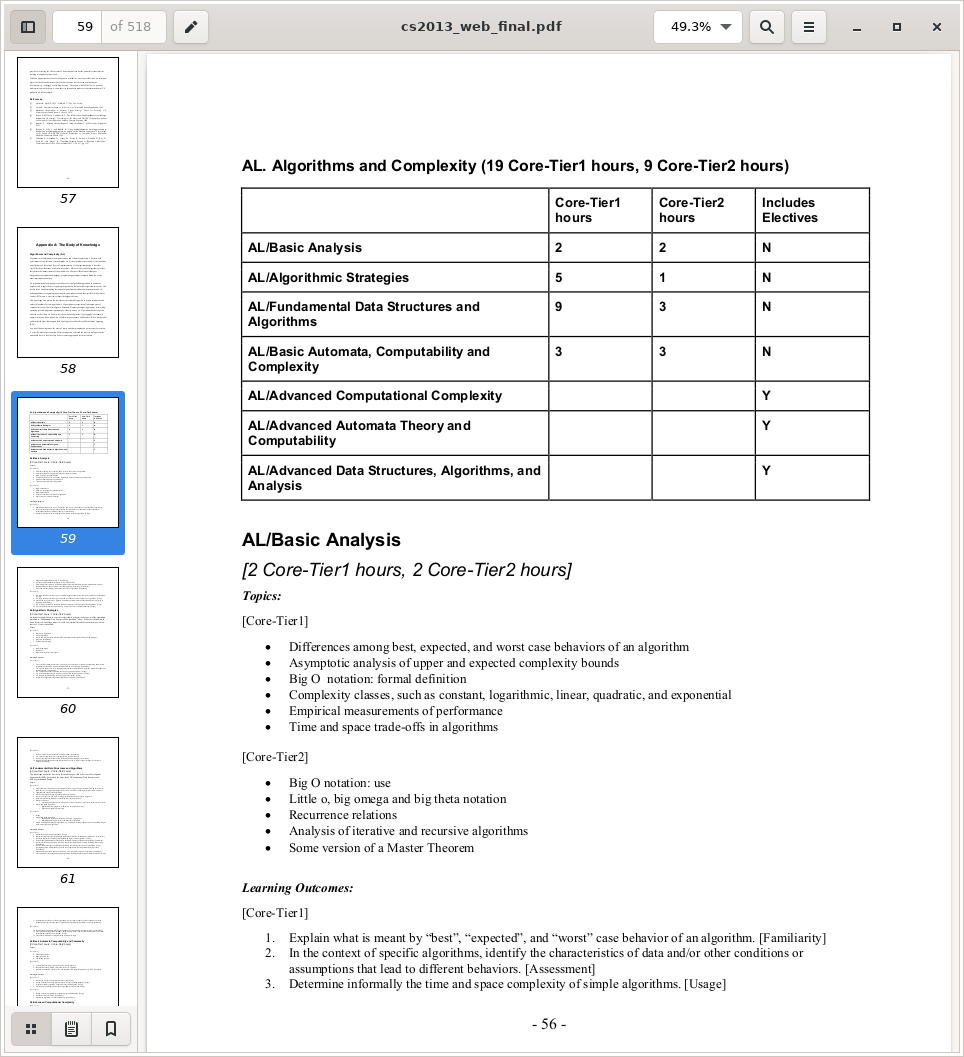
\includegraphics[width=\linewidth]{figs/cs2013-ALpage1.png}

  \end{columns}
\end{frame}

\begin{frame}
  \frametitle{Specific Guidelines: NSF/IEEE-TCPP PDC 2012}

  Structured in domains:
  \begin{itemize}
  \item Programming
  \item Algorithm
  \item Architecture
  \end{itemize}

  More descriptive.

  Bloom levels.

  Other specific guidelines: graphics, security  
\end{frame}


\begin{frame}
  \frametitle{Activity}

  \begin{itemize}
  \item Look at the ACM/IEEE CS 2013 guidelines.
  \item Find some entries relevant to one of your course.
  \item But also browse it to get a sense of the scope of it.
  \item Notice the examplar at the end. Find and read through an examplar for
    a course similar to what you teach.
  \end{itemize}
\end{frame}

\subsection{What do other instructors do in their course?}

\begin{frame}
  \frametitle{A Lingua Franca}

  CS Guidelines give us a fairly detailed description of what is in CS.

  We can use them as ontologies to describe in a common language what
  a course of a class material is like.

  \begin{block}{What do you think is in a lecture entitled UNCC-ITCS-2214-Saule-Graphs?}
    \tiny
  \begin{itemize} 
    \item Depth- and breadth-first traversals
    \item Representations of graphs (e.g., adjacency list, adjacency matrix)
    \item Reflexivity, symmetry, transitivity
    \item Illustrate by example the basic terminology of graph theory, and some of the properties and special cases of each type of graph/tree.
    \item Undirected graphs
    \item Directed graphs
    \item Weighted graphs
    \item Iterative and recursive traversal of data structures
  \end{itemize}
  \end{block}
\end{frame}

\begin{frame}
  \frametitle{Study of Coverage}

  We can easily understand what one course is covering.

  We can understand across multiple offfering of the same course what that particular course is about.

  We can identify different ``flavors'' of that course.  
\end{frame}

\begin{frame}
  \frametitle{Activity}

  Look at the different data structure course using the coverage map.

  For a particular course:
  \begin{itemize}
  \item Note something they are teaching and that you were not expecting.
  \item Note something you thought they would cover and are not covering
  \end{itemize}

  Look at all courses at once:
  \begin{itemize}
  \item What are the key topics/outcome that are covered by most?
  \end{itemize}
\end{frame}

\subsection{Principles of Alignment}

\begin{frame}
  \frametitle{What is Alignment?}

  \begin{block}{Properties of how content flow in}
    \begin{itemize}
    \item Program
    \item Course
    \item Module
    \end{itemize}
  \end{block}

  \begin{block}{That could apply to}
    \begin{itemize}
    \item Topics
    \item Outcomes
    \item Competencies
    \end{itemize}
  \end{block}

  \begin{block}{That could be in term of}
    \begin{itemize}
    \item What they cover
    \item What they assume students know
    \end{itemize}
  \end{block}
  
\end{frame}

\begin{frame}
  \frametitle{Aligning Modules with Course Objectives}
    Courses usually have objectives that come from program
    descriptions and assessments.

    How do we ensure that the content of the class actually serve
    these higher objective? We want to align the objective modules
    with the objective of the course.

    Two main properties to check:
    \begin{itemize}
    \item Are all the course objectives covered appropriately by a module objective?
    \item Are there module objectives that serve no course objective?
    \end{itemize}

\end{frame}

\begin{frame}
  \frametitle{Alignment within Module}

  \begin{block}{Typical module structure}
    \begin{itemize}
    \item Exposition to new concept (lecture, textbook)
    \item Clarification of concept (discussion, hands-on activity)
    \item Reinforcement of concept (problem, programming assignment)
    \end{itemize}
  \end{block}
  
  \begin{block}{Properties you want}
    \begin{itemize}
    \item The clarification should not introduce new concepts
    \item The reinforcement should strengthen the exposition and clarification topics
    \item The materials should cover the topics the module is meant to cover
    \item The materials should not wander too far from the module objectives
    \end{itemize}
  \end{block}

  \begin{block}{Assessment}
    Exam should never introduced new concepts
  \end{block}  
\end{frame}

\begin{frame}
  \frametitle{Activity}

  \begin{block}{For a particular course, look at the lectures and assignment}
    
    \begin{itemize}
    \item Are there topics in the assignment that are not part of the lecture?
      \begin{itemize}
      \item Do you think it is a problem?
      \end{itemize}
    \item Are there topics in the lecture that are not in the assignment?
      \begin{itemize}
      \item Do you think it is a problem?
      \end{itemize}
    \end{itemize}
    
  \end{block}
  
  \begin{block}{Consider two sections of data structures}
    \begin{itemize}
    \item Can you identify differences between the two sections
      \begin{itemize}
      \item Are any of this difference style or fundamental?
      \end{itemize}
    \end{itemize}
  \end{block}
\end{frame}

\subsection{Searching for content}

\begin{frame}
  \frametitle{Have you ever searched for materials?}

  Let's look at Nifty Assignments

  \begin{columns}
    \column{.49\linewidth}
    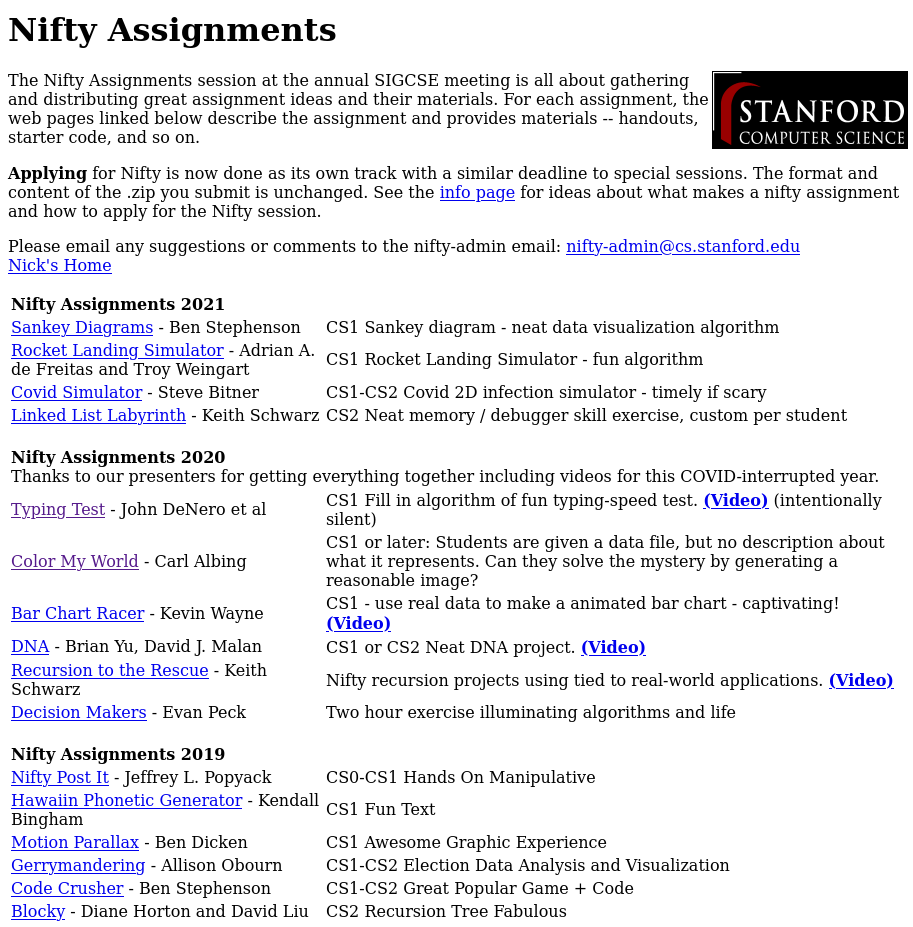
\includegraphics[width=\linewidth]{figs/Nifty.png}
    
    \column{.49\linewidth}
    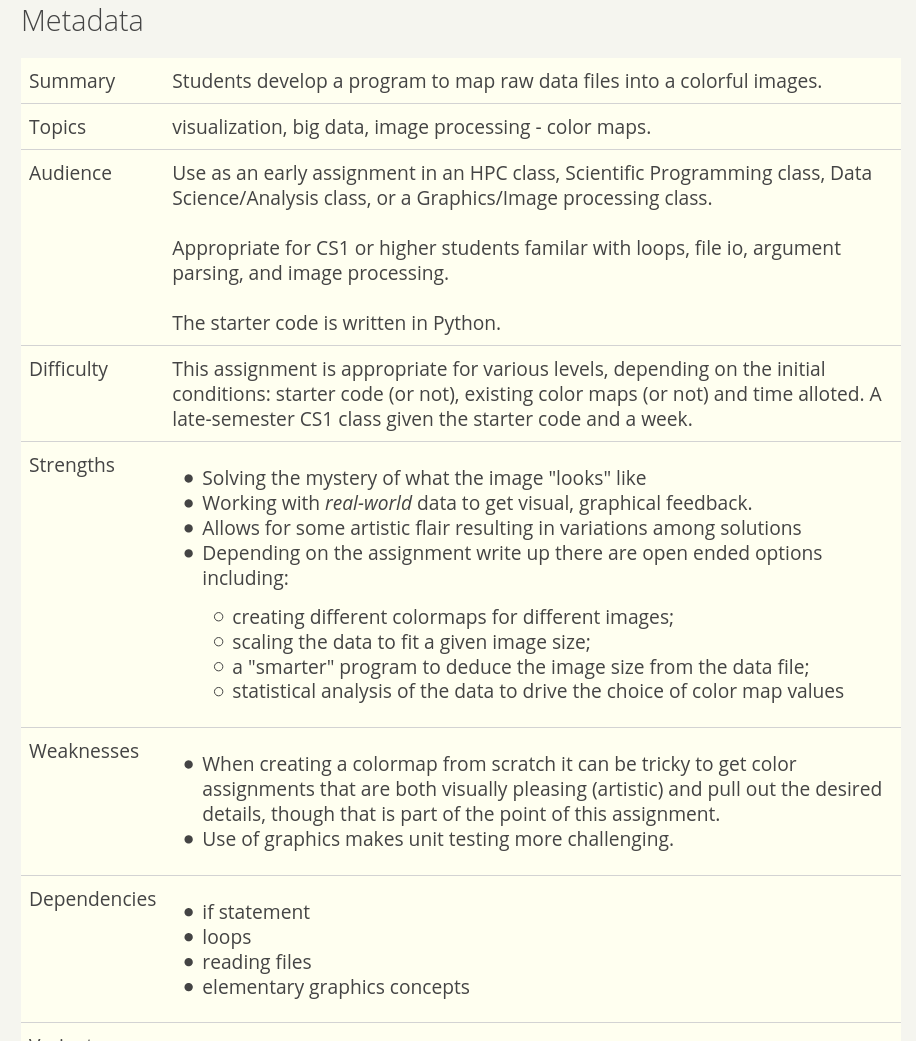
\includegraphics[width=\linewidth]{figs/AParticularNifty.png}
  \end{columns}
  
\end{frame}

\begin{frame}
  \frametitle{Curriculum Guidelines as Features}

  \begin{block}{Features}
    The problem in classic search is that it is hard to find good
    matches because people use imprecise textual descriptions.

    Curriculum guidelines give us a well established precise features
  \end{block}

  \begin{block}{Search}
    Give a set of materials that use these topics/outcomes
  \end{block}

  \begin{block}{Recommendation}
    Give a set of materials that match the same outcomes as these ones.
  \end{block}
  
\end{frame}

\begin{frame}
  \frametitle{Activity}

  Can you find materials about hash tables?

  Can you find materials about shortest path?
\end{frame}


\end{document}
%
